\chapter{Critical Evaluation}
\label{chap:evaluation}

\section{Analysis of Word Lists}
\label{sec:word-list-analysis}
\begin{figure}[ht]
\begin{subfigure}[b]{\textwidth}
\centering
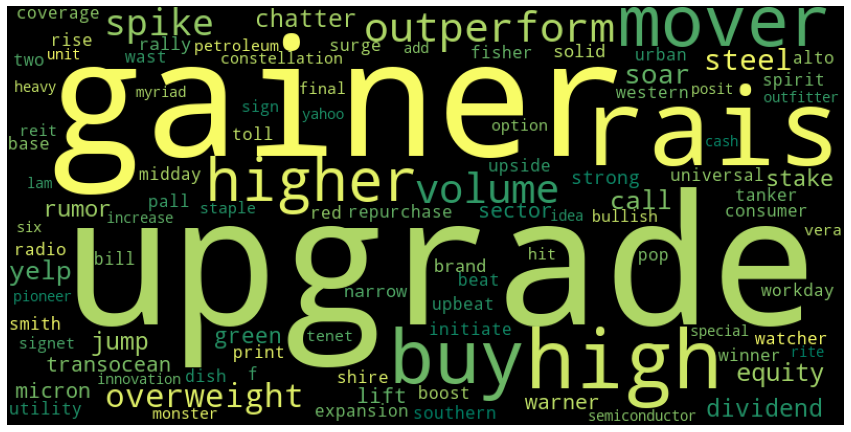
\includegraphics[scale=0.4]{pics/positive.png}
\caption{Positive words}
\end{subfigure}

\begin{subfigure}[b]{\textwidth}
\centering
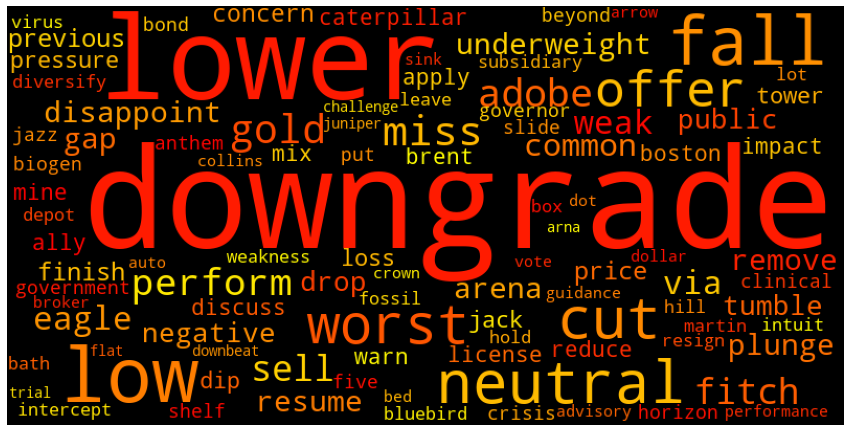
\includegraphics[scale=0.4]{pics/negative.png}
\caption{Negative words}
\end{subfigure}
\caption[Word clouds]{Word clouds demonstrating sentiment charged words. Font size corresponds to average tone across all training samples}
\label{wordclouds}
\end{figure}

Following the construction of matrix $O$, figure \ref{wordclouds} demonstrates the list of sentiment charged words on average over all training 19 windows. At each training and validation window, the sentiment lists are generated completely from scratch, and while there is some overlap, each list can vary significantly. The font size corresponds to the average tone (calculated by $\frac{1}{2}(O_+ - O_-)$) of the words across all windows. Of the top 50 positive sentiment words, the following appeared in at least 15 of the 19 windows, with words highlighted in \textbf{bold} appearing in all windows:
\begin{center}
      \textit{author, rumor, volume, repurchase, rais(e),} \textbf{gainer, mover, high, upgrade}
\end{center}

\noindent
The following words appear in at least 15 of the 19 windows with respect to top 50 negative sentiment words with those highlighted in \textbf{bold} appearing in all windows:
\begin{center}
      \textit{offer, negative, neutral, public, low,} \textbf{miss, lower, loser, cut, fall, weak, downgrade, underweight}
\end{center}

Simply by inspection, each group appears reasonable, in the sense that many of the words with high values in either sentiment could be assumed. However, some words are somewhat surprising and this may offer an insight into subconscious bias that exists in writing headlines as opposed to article bodies. For example, the word \textit{volume} is, under normal circumstances, a sentiment neutral word, but according to the model generated by SESTM, is a highly positive word. Examples of headlines including this word include:
\begin{itemize}
      \item \textit{Agilent spikes to high of \$60.40 on Volume}
      \item \textit{Markets gather some momentum as volume remains light, geopolitical tension improving}
      \item \textit{Tuesday's Mid-day options for volume leaders}
\end{itemize}

Observing these headlines, it is clear that the words are being used in a positive context, and this could be due to subconscious usage of the word when constructing such headlines. However, in any learning based algorithm, overfitting must be considered. Overfitting in this instance refers to a model that is too closely trained to the training sample, meaning incorrect alignment with out of sample data. Included in the sample are headlines from `Benzinga', which is a company that offers realtime news articles \parencite{benzinga-website}, and has a significant quantity of headlines of the form \textit{Benzinga's top upgrades} (around 16,000 headlines from the entire dataset) and \textit{Benzinga's volume} (with around 2,000). To account for this, the addition of bigrams (discussed further in \ref{sub:bigram-analysis}) gives an insight into frequently occurring pairs of words, and helps to isolate context specific sentiment. If a word has a high estimated impact in a bigram, then the majority of the sentiment comes from its co-appearance with its partner word, helping to eliminate such issues.

Some words, such as `rais' are cut off to their stem by the stemming and lemmatisation step (i.e. `rais' from `raise'), as the stem is also an English word. However, such words are likely to be very infrequently used words themselves, and are very unlikely to be used in a headline. These edge cases do not affect the overall predictive quality of the model, as evidenced by the words shown in figure \ref{wordclouds}. The sentiment for each word is still captured in the stem, and each article is processed in the same way, thus there is no sentiment or predictive power lost in this way. There is a slight complication when it comes to comparing the words included in the model to those in the H4 and LM lexicons, as these lexicons do not contain the stemmed words. For this reason, when checking if a word in the trained model exists in either dictionary, each word in either dictionary is preprocessed in the same way discussed in section \ref{sec:pre-processing}

When compared to the Harvard IV and Loughran McDonald dictionaries, we find that the majority of words labelled with sentiment according to our model are not in either dictionary. The negative sentiment words have much higher overlap, with 13 of the top 50 words appearing in the LM dictionary, while only 3 appear in the H4. Conversely, only 6 words overlap LM in the positive tone, while 5 words overlap the H4 dictionary. Furthermore, many words that are included in either dictionary are determined to be sentiment neutral by the model. This is because the model is trained on a sample of headlines and the vocabulary used in headlines is vastly different to that in everyday use or 10-k filings in the case of LM. Headline vocabulary often contains much more impactful words, as it is intended to be a punchy, attention grabbing piece of text. Often, words that are typically used in headlines are rarely found outside of the context of headlines \parencite{language-newspapers}. For this reason, the lexicons of the model, and that of H4 and LM differ significantly.

\subsection{Bigrams}
\label{sub:bigram-analysis}
The order in which words appear in can have a profound effect on the sentiment of a word. This order sentiment can be captured by exploring the dictionary when constructed from \textit{bigrams} as opposed to unigrams alone. By combining both of these dictionaries, it is possible to gain a clearer understanding of the true sentiment of a headline. Many of the frequently  words unigrams also appear in the bigram. This is partly due to the mutual information restriction on the bigrams consiered by the model, but also because still carry sentiment in combination with other words. Furthermore, somewhat surprisingly there are bigrams that appear in every training window. The headlines in this dataset have an average wordcount of 6.11 (excluding stopwords and non-English words), and therefore one may expect that there would be very few repeating bigrams, which is not the case. This signifies that headline writers may subconsciously use certain combinations of words to convey either positive or negative sentiment

The following bigrams appear positively in at least 13 of the 19 training windows, with those highlighted in \textbf{bold} appearing in all headlines:
\begin{center}
\textit{micron technology, repurchase program, spike higher,} \textbf{volume mover}, \textbf{week high}
\end{center}

The following bigrams appear negatively in at least 14 of the 19 training windows, with those highlighted in \textbf{bold} appearing in all headlines:
\begin{center}
      \textit{general dynamic, bath beyond, bed bath, sector perform, secondary offer, week low, resume trade, offer common,} \textbf{public offer}
\end{center}

Several of the high frequency unigrams do not appear in the high frequency bigrams, indicating that the sentiment carried by these words is not tied to context, for example raise for positive and weak for negative. Due to the nature of the headlines, the model also picks up on especially highly or poorly performing companies, and this is sometimes reflected in the generated word lists. For example, `\textit{bed bath}' and `\textit{bath beyond}' both appearing in the negative bigram list is almost certainly a result of the poor performance of the company \textit{Bed, Bath and Beyond}, whose stock prices stagnated and then fell from mid 2013 \parencite{bed-bath-yahoo}. Also seen in figure \ref{wordclouds}, Adobe is likely to be in reference to the company `Adobe'.


\section{Daily returns}
\label{sec:daily-returns-analysis}

\begin{table}[!ht]
\begin{center}
\begin{tabular}{lccccccc}
      \toprule
      & Sharpe &  Average & Daily & \multicolumn{2}{c}{FF3} & \multicolumn{2}{c}{FF5} \\
      \cmidrule(lr){5-6}
      \cmidrule(lr){7-8}
      % \cmidrule(lr){9-10}
      Formation & Ratio & Return & Turnover & $\alpha$ & $R^2$ & $\alpha$ & $R^2$ \\
      \midrule
      EW LS & 0.84 & 9.23 & & 5.59 & 4.11\% & 5.57 & 4.16\% \\
      EW L & 0.69 & 9.75 & & 6.56 & 21.62\% & 5.86 & 23.0\% \\
      EW S & -0.09 & -0.53 & & -1.66 & 25.71\% & -0.98 & 26.68\% \\
      VW LS & 0.56 & 6.31 & & 4.73 & 0.83\% & 7.16 & 4.58\% \\
      VW L & 0.86 & 10.47 & & 6.51 & 34.3\% & 7.55 & 35.16\% \\
      VW S & -0.38 & -4.16 & & -2.48 & 32.54\% & -1.08 & 34.08\% \\
      \bottomrule
\end{tabular}
\caption{Performance of Daily News Sentiment Portfolios one day ahead}
\label{portfolio-performance}
\end{center}
\end{table}

Using the headlines that were saved for out of sample testing, a portfolio is constructed for each day. On average, 358 firms have articles linked to them on a given day, and of these, almost three quarters of these firms have headlines containing one or more sentiment words (are not marked neutral by the model). According to the constraints ($\widehat p_i < 0.5$ for a stock to be bought, and vice versa for a stock to be sold), there are some days where less than 100 stocks form the portfolio, in which case we trade with the largest value possible. On average, the long side trades with 49.5 stocks, while the short side has 48, so the model trades at very close to 100 stocks the majority of the time.

Table \ref{portfolio-performance} describes the performance of the constructed portfolios. The long-short portfolio is a zero-net-investment portfolio, which is a theoretical portfolio that requires zero investment, as it buys the same value of stocks as it sells \parencite{zero-net}. The portfolio is theoretical as a true zero-cost investment is impossible in practice for a number of reasons, one of which being that to sell a stock and profit from the decline, there is collateral from the loan from the broker. However, for the purposes of the following experiments, it is sufficient. The two investment methods (equal and value weighted) are split up into the long-short combined portfolio (L-S), and the long (L) and short (S) legs are also displayed separately for comparison purposes. The daily turnover section displays the average turnover each day, which would be 100\% as the profit is liquidated at the end of each day, but some stocks are retained the following day. A turnover of 90\% (as in VW L) implies that on average 1 in 10 stocks are retained the following day. This could be due to headlines or news articles that are concerning the same events (stale news), or repeat sentiment headlines as a story unfolds over a number of days.

The Sharpe ratio refers to the calculated annualised sharpe ratio and this reflects the ratio of profit versus risk. Sharpe ratios are annualised by multiplying the daily sharpe ratio (shown in \ref{ssub:sharpe-ratio}) by $\sqrt{252}$ as this is the number of trading days in a year, and will give a clearer image of the risk involved in the potential profit.

The FF3 and FF5 sections refer to Fama French 3 and 5 factor regression respectively, while the $\alpha$ concerns the intercept. The $\alpha$ value reflects how much the output outperformed the expected value calculated by the factors in the model and is generated by privately created information, or information that is not available in the market. In other words, if the $\alpha$ is a very small percentage of the generated returns, then the returns that an investment has generated can be explained by regular movement in the markets, and there is no private information that is being used to generate profit. The $R^2$ value is the measure of the proportion of variance that is for the dependent variable (in this case, daily returns for the portfolio) is explained by the independent variables (in this case, the Fama French factors discussed in \ref{ssub:fama-french}). Therefore, if $R^2 = 25\%$, then around a quarter of the observed variation can be explained by the inputs. In terms of an investment, this corresponds to the percentage of movement that can be explained by movements in the independent variables.

This figure clarifies two key facts: firstly, most of the formations generate a slight profit with a fair amount of risk, reflected in the Sharpe ratios. None of the formations have a Sharpe ratio of $>1$, meaning each of the portfolios carry significant risk. The second fact is that the equal weighted portfolio outperforms the value weighted portfolio overall, while the value weighted portfolio sees a slight performance on the long side.

\begin{figure}[!t]
      \centering
\begin{tikzpicture}
\begin{axis}[scale only axis, height=8cm, width=\textwidth*.9, grid=both,
      legend pos=north west,
      date coordinates in=x, date ZERO=2019-01-01, xticklabel=\month-\year,ymin=-50,ymax=75,
      xtick={2019-01-01,2019-02-01,2019-03-01,2019-04-01,2019-05-01,2019-06-01,2019-07-01,2019-08-01,2019-09-01,2019-10-01,2019-11-01,2019-12-01,2020-01-01,2020-02-01,2020-03-01,2020-04-01,2020-05-01,2020-06-01},
      xticklabel style={
            rotate=60,
      },
       xmin=2019-01-01,
       xmax=2020-06-08]
\addplot [red, very thick, mark=none] table [header=true,x=date,y=EW-L, col sep=comma]{data/one-day-ahead.csv};
\addplot [blue, very thick, mark=none] table [header=true,x=date,y=EW-S, col sep=comma]{data/one-day-ahead.csv};
\addplot [black, very thick, mark=none] table [header=true,x=date,y=EW-LS, col sep=comma]{data/one-day-ahead.csv};
\addplot [red, very thick, dotted, mark=none] table [header=true,x=date,y=VW-L, col sep=comma]{data/one-day-ahead.csv};
\addplot [blue, very thick, dotted, mark=none] table [header=true,x=date,y=VW-S, col sep=comma]{data/one-day-ahead.csv};
\addplot [black, very thick, dotted, mark=none] table [header=true,x=date,y=VW-LS, col sep=comma]{data/one-day-ahead.csv};
% \draw ({axis cs:2020-03-11,0}|-{rel axis cs:0,0}) -- ({axis cs:2020-03-11,0}|-{rel axis cs:0,1})
 \draw[green, very thick] (axis cs: 2020-03-11,\pgfkeysvalueof{/pgfplots/ymin}) -- 
                      (axis cs: 2020-03-11,\pgfkeysvalueof{/pgfplots/ymax})node[anchor=west,rotate=90]{Coronavirus declard pandemic};
                
\legend{L EW, S EW, LS EW, L VW, S VW, LS VW}

\end{axis}
\end{tikzpicture}
\caption[Daily cumulative log returns]{Cumulative log returns for each formation over the out of sample headlines}
\label{graph-returns}
\end{figure}


Figure \ref{graph-returns} details the cumulative log returns over the entire out of sample dataset. Here, The performance of each of the legs are relatively steady in their respective directions until March 2020. At this point, the profits of the short legs skyrocket, while that of the long section plummet --- especially for the value weighted portfolios. This is due to the Coronavirus outbreak, as it was officially declared a pandemic on March 11 2020, indicted by the vertical green line on the graph. Due to lockdown restrictions imposed wordwode, the stock market experienced one of the worst crashes, and was felt particularly by large stocks, before recovering a short while later. The markets began feeling the effect of the lockdown in February 2020, and the crash peaked in March 2020, before beginning to recover in late April \parencite{covid-impact}. This crash can be clearly seen in the affected profits, as the long side suffers significantly, while the short side succeeds greatly. This is simply due to the vasy majority of stocks falling in value, therefore shorting almost any stocks during this time would result in a profit. The extreme disparity in profit for the long side also clearly highlights a limitation with all lexicon based sentiment analysis methods, whether they use supervised learning signals, or use a manually labelled dictionary: they are unable to adapt to rapid changes. Since the COVID-19 virus did not exist during the training and validation samples, the model has no information on the sentiment of headlines that would discuss this, and would ignore it. Naturally, if the model was retrained using data from this time period, it would be able to detect such headlines in the future, but the crux of the issue is that it is impossible to obtain enough information to allow the model to react to such drastic changes in the market.

Graph \ref{graph-returns} reveals slightly different information than that in table \ref{portfolio-performance}. Here, the long side of the value weighted graph is shown to outperform the equal weighted counterpart considerably, before taking a substantial fall during the pandemic induced market crash. On the other hand, the short sides of both weighting strategies fare similarly, until after the crash, where the equal weighted short side experiences a higher spike in profit. Clearly, SESTM is capable of predicting a positive shift in stocks on a one-day-ahead principle, shown by the positive returns in the graph. It is more successful when predicting larger stocks, as value weighed portfolios are influenced more by larger stocks. This represents SESTM's success in detecting positive sentiment in headlines concerning these large firms, which is likely due to increased coverage. As previously discussed, the primary goal for a headline is to capture as much information about the main article body as possible while the secondary goal is to attract the reader to click on the article. For this reason, the headline is far more likely to contain information about more well known stocks, as this satisfies the secondary goal of garnering clicks: if the headline's content is about a stock that is known to the reader, it is more likely that the rest of the article is read.

The two short formations perform very similarly, with both making slight losses. This contradicts the claims made concerning headlines containing more information about large stocks somewhat, although I believe this is due to a different matter. \textcite{linguistic-effect-success} explore the success of a headline based on linguistic features, and conclude that the presence of positive-emotion words is negatively associated with the success of a headline (in terms of popularity), while the inverse is true for negative-emotion words. For this reason, if there is ambiguity on the potential future of a stock, a headline is more likely to take the negative approach, as it is more likely to be successful. In other words, if a news article is mostly neutral, the headline is more likely to contain negative-emotion words, as this garners more views. As a result, the negatively tagged words are less reliable than their positive tagged counterparts, which be one possbile explanation for the lack of profit made by either short formation.

\begin{table}[!ht]
\begin{center}
\begin{tabular}{lccccccc}
      \toprule
      & Sharpe &  Average & Daily & \multicolumn{2}{c}{FF3} & \multicolumn{2}{c}{FF5} \\
      \cmidrule(lr){5-6}
      \cmidrule(lr){7-8}
      Formation & Ratio & Return & Turnover & $\alpha$ & $R^2$ & $\alpha$ & $R^2$ \\
      \midrule
      EW LS & 0.84  & 9.23 & & 5.59 & 4.11\% & 5.57 & 4.16\% \\
      EW L  & 0.69  & 9.75 & & 6.56 & 21.62\% & 5.86 & 23.0\% \\
      EW S  & -0.09 & -0.53 & & -1.66 & 25.71\% & -0.98 & 26.68\% \\
      VW LS & 0.56  & 6.31 & & 4.73 & 0.83\% & 7.16 & 4.58\% \\
      VW L  & 0.86  & 10.47 & & 6.51 & 34.3\% & 7.55 & 35.16\% \\
      VW S  & -0.38 & -4.16 & & -2.48 & 32.54\% & -1.08 & 34.08\% \\
      \midrule
      \multicolumn{8}{c}{Excluding market crash} \\
      \midrule
      EW LS & 0.66  & 6.51 & & 5.52 & 2.24\% & 4.16 & 4.51\% \\
      EW L  & 0.64  & 5.46 & & 1.95 & 9.67\% & 0.58 & 12.97\% \\
      EW S  & 0.03  & 1.05 & & 2.76 & 16.16\% & 2.77 & 16.96\% \\
      VW LS & 0.99  & 7.61 & & 6.46 & 0.81\% & 6.67 & 0.9\% \\
      VW L  & 1.52  & 10.98 & & 7.95 & 14.51\% & 7.84 & 14.59\% \\
      VW S  & -0.59 & -3.37 & & -2.3 & 17.95\% & -1.98 & 18.21\% \\
      \bottomrule
\end{tabular}
\caption{Performance of daily news sentiment portfolios one day ahead, ignoring headlines dated after January 2020}
\label{tab:portfolio-performance-no-covid}
\end{center}
\end{table}

For closer inspection of the model's predictive ability, table \ref{tab:portfolio-performance-no-covid} shows the same metrics as table \ref{portfolio-performance}, only without any of the out of sample articles dated after February 28th 2020 to observe the impact without the greatly added noise of a stock market crash. Here, the trend of the data is very similar, with the value weighted long formation still outperforming its equal weighting counterpart, and vice versa with the short side, meaning that it remains steadfast that headlines indicating negative sentiment about smaller stocks contain more reliable information than that with positive stocks. The most notable increase in Sharpe ratio is the value weighted long side, despite only a marginal increase in average return. This is likely due to the large plunge in prices shortly after the global pandemic announcement, which increases the standard deviation of the portfolio significantly, thus increasing perceived risk. Other than this formation, it is clear to see that the model struggles to see any profit devoid of serious risk, indicated by all Sharpe ratios being $<1$. Headlines being so short in terms of word count, as well as the small out of sample dataset size, lead to difficulties in gaining sufficient information to consistently accurately predict stock movement based on headlines alone. The conclusions drawn from headlines leave large room for error and while there is still potential for information gain, the signal is not as clear as longer text forms.

\begin{table}[!ht]
\begin{center}
\begin{tabular}{l|cc|ccccccc}
      \toprule
      & Baseline & Baseline& Sharpe &  Average & Daily & \multicolumn{2}{c}{FF3} & \multicolumn{2}{c}{FF5} \\
      \cmidrule(lr){7-8}
      \cmidrule(lr){9-10}
      % \cmidrule(lr){9-10}
      Formation & Sharpe & Returns & Ratio & Return & Turnover & $\alpha$ & $R^2$ & $\alpha$ & $R^2$ \\
      \midrule
 EW LS & 0.84  & 9.23 & 1.75 & 20.69 & & 18.19 & 8.87\% & 17.71 & 8.98\% \\
 EW L  & 0.69  & 9.75 & 1.29 & 17.84 & & 14.55 & 18.81\% & 14.02 & 19.93\% \\
 EW S  & -0.09 & -0.53 & 0.15 & 2.85 & & 2.95 & 34.48\% & 3.0 & 35.2\% \\
 VW LS & 0.56  & 6.31 & 1.62 & 15.45 & & 12.45 & 5.12\% & 13.41 & 6.31\% \\
 VW L  & 0.86  & 10.47 & 1.01 & 11.32 & & 8.21 & 32.42\% & 9.13 & 33.53\% \\
 VW S  & -0.38 & -4.16 & 0.27 & 4.13 & & 3.55 & 30.11\% & 3.58 & 31.48\% \\
 \midrule
 \multicolumn{10}{c}{Excluding market crash} \\
 \midrule
 EW LS & 0.66  & 6.51 & 0.85 & 8.26 & & 7.15 & 2.49\% & 6.09 & 3.77\% \\
 EW L  & 0.64  & 5.46 & 1.12 & 9.19 & & 5.86 & 9.2\% & 4.79 & 11.25\% \\
 EW S  & 0.03  & 1.05 & -0.21 & -0.93 & & 0.47 & 16.02\% & 0.49 & 16.59\% \\
 VW LS & 0.99  & 7.61 & 1.53 & 11.16 & & 10.54 & 1.43\% & 10.78 & 1.54\% \\
 VW L  & 1.52  & 10.98 & 1.35 & 9.93 & & 7.07 & 17.33\% & 7.15 & 17.46\% \\
 VW S  & -0.59 & -3.37 & 0.06 & 1.23 & & 2.66 & 21.48\% & 2.81 & 21.59\% \\
      \bottomrule
\end{tabular}
\caption[Day ahead performance with bigrams]{Performance of daily news sentiment portfolios using bigrams alongside unigrams. Baseline values are those achieved by unigrams alone}
\label{tab:other-configs-day-ahead}
\end{center}
\end{table}

Table \ref{tab:other-configs-day-ahead} shows the performance of the portfolios when augmenting the sentiment word list with bigrams. Most notable in this table is the vast improvement in both sharpe ratios and the average daily returns for the equal weighted strategy, particularly in the long leg of the portfolios. The sharpe ratio of 1.75 produced by the equal weighted portfolio shows that the profit generated has a very favourable risk to profit ratio. This large shift in performance indicates that sentiment in headlines as a whole is often conveyed using multiple words, and that context has importance in this text type. Ignoring articles from after the market crash, the performance of all formations is either comparable or better, reinforcing this notion. As before, a very high proportion of returns are alhpa, meaning private information not available to the market is present in this model.

%note!: alpha for 

%todo: do portfolios trading 200 stocks also to show robustness
\section{Speed of information Assimilation}
\label{sec:speed-assim}

In the previous sections, we explore the relationship between the sentiment score of a headline calculated by the model and the changes in price the following day. Here, we explore the relationship between the changes in price after differing delays to investigate timing responses.

\begin{table}[!t]
\begin{center}
\begin{tabular}{lccccccc}
      \toprule
      & Sharpe &  Average & Daily & \multicolumn{2}{c}{FF3} & \multicolumn{2}{c}{FF5} \\
      \cmidrule(lr){5-6}
      \cmidrule(lr){7-8}
      % \cmidrule(lr){9-10}
      Formation & Ratio & Return & Turnover & $\alpha$ & $R^2$ & $\alpha$ & $R^2$ \\
      \midrule
      \multicolumn{8}{c}{Day $t-1$} \\
EW LS & 15.48 & 210.11 & & 207.8 & 1.09\% & 207.19 & 4.93\% \\
EW L & 7.83 & 122.42 & & 120.91 & 21.43\% & 120.44 & 23.06\% \\
EW S & 5.87 & 87.7 & & 86.2 & 28.81\% & 86.05 & 29.01\% \\
VW LS & 9.27 & 110.04 & & 107.9 & 1.22\% & 108.69 & 3.74\% \\
VW L & 4.18 & 55.35 & & 52.18 & 34.77\% & 52.99 & 36.55\% \\
VW S & 4.55 & 54.69 & & 55.02 & 31.73\% & 54.99 & 31.75\% \\
      \multicolumn{8}{c}{Day $t+0$} \\
EW LS & 15.67 & 234.84 & & 233.93 & 2.46\% & 233.89 & 3.05\% \\
EW L & 7.57 & 134.7 & & 134.21 & 10.26\% & 134.64 & 11.18\% \\
EW S & 6.21 & 100.15 & & 99.03 & 21.85\% & 98.56 & 22.02\% \\
VW LS & 12.51 & 139.79 & & 139.08 & 1.39\% & 139.21 & 1.62\% \\
VW L & 3.77 & 53.24 & & 51.09 & 15.87\% & 51.56 & 17.01\% \\
VW S & 6.87 & 86.55 & & 87.3 & 24.3\% & 86.96 & 24.89\% \\
      \multicolumn{8}{c}{Day $t+1$} \\
EW LS & 0.84 & 9.23 & & 5.59 & 4.11\% & 5.57 & 4.16\% \\
EW L & 0.69 & 9.75 & & 6.56 & 21.62\% & 5.86 & 23.0\% \\
EW S & -0.09 & -0.53 & & -1.66 & 25.71\% & -0.98 & 26.68\% \\
VW LS & 0.56 & 6.31 & & 4.73 & 0.83\% & 7.16 & 4.58\% \\
VW L & 0.86 & 10.47 & & 6.51 & 34.3\% & 7.55 & 35.16\% \\
VW S & -0.38 & -4.16 & & -2.48 & 32.54\% & -1.08 & 34.08\% \\
      \bottomrule
\end{tabular}
\caption{Performance of Daily News Sentiment Portfolios day $t-1$ to day $t+1$}
\label{portfolio-performance-day-1}
\end{center}
\end{table}

Table \ref{portfolio-performance-day-1} portays the returns of different holding lengths on returns. For day $t-1$ and $t+0$, these are purely theoretical and serve only as an insight into the models performance. The day $t+1$ section shows the same information as \ref{portfolio-performance} as a reference.

The day $t-1$ section explores portfolios created the day before a headline is released. The portfolios are constructed in the same manner as table \ref{portfolio-performance}, however, the theoretical portfolios crafted here are based on the sentiment headlines that have not yet been released. By doing so, we investigate how estimated sentiment score $\widehat p_i$ picks up on stale news. This is reflected in the entirely infeasible Sharpe ratios of 15.48 and 10.8 for equal and value weighted portfolio formations respectively.

The day $t + 0$ section explores a portfolio crafted on the same day as the headline is released, providing an insight into how the estimated sentiment score picks up on fresh news. This method sees the largest profit of any formation, indicating that the freshness of news is significant when observing sentiment. In other words, the closer to the release of a headline that the sentiment can be utilised, the greater the potential profits.
\begin{figure}[!ht]
      \centering
\begin{tikzpicture}
\begin{axis}[scale only axis, height=8cm, width=\textwidth*.9, grid=both,
      legend columns=2,
      % legend style={
      %       /tikz/column 2/.style-{
      %             column sep=5pt,
      %       },
      % },
      legend pos=north east,
      ymin=-15,ymax=20,
      xtick={1,2,3,4,5,6,7,8,9,10},
      xticklabels={Day+1, Day+2,Day+3,Day+4,Day+5,Day+6,Day+7,Day+8,Day+9,Day+10},
      xmin=1,
      xmax=7]
\addplot [black, very thick, mark=x] table [header=true,x=day,y=avg-LS, col sep=comma]{data/speed-assimilation.csv};
\addplot [black, very thick, dotted, mark=x] table [header=true,x=day,y=avg-LS-no-covid, col sep=comma]{data/speed-assimilation.csv};
\addplot [red, very thick, mark=x] table [header=true,x=day,y=avg-L, col sep=comma]{data/speed-assimilation.csv};
\addplot [red, very thick, dotted, mark=x] table [header=true,x=day,y=avg-L-no-covid, col sep=comma]{data/speed-assimilation.csv};
\addplot [blue, very thick, mark=x] table [header=true,x=day,y=avg-S, col sep=comma]{data/speed-assimilation.csv};
\addplot [blue, very thick, dotted, mark=x] table [header=true,x=day,y=avg-S-no-covid, col sep=comma]{data/speed-assimilation.csv};
\legend{L-S, L-S (no-covid), L, L (no-covid), S, S (no-covid)}
\end{axis}
\end{tikzpicture}
\caption[Graph of average daily returns for different waiting periods]{Average daily returns for different waiting periods. If article is released on day $t$ (between 9 a.m. of day $t$ and 9 a.m. of day $t+1$), portfolio is created on day $t+n$ and sold on day $t+(n+1)$ where $n$ is the value indicated by the x axis}
\label{fig:speed-assimilation}
\end{figure}

Figure \ref{fig:speed-assimilation} shows the time taken for a headline to be fully assimilated into the stock prices. The graph indicates that SESTM picks up on sentiment that takes a few days to be fully incorporated into the prices, as it takes until day $+ 5$ for the LS portfolio to reach zero. The short side is incorporated much more quickly, only taking around 2 days to be fully assimilated, while the long side takes around 5 days for full assimilation. The information shown by this graph is important as it can potentially show that a portfolio is able to pick up on complex sentiment that takes a number of days to fully assimilate into the prices.


\section{Comparison to other methods}
\label{sec:comparison}
%todo plot log cum returns of lm and h4 compared to sestm
%TODO create table of regression on LM and H4 dictionaries to show information not captured by each

In this section, we compare the ability of SESTM against similar strategies. Similar to the methods used to construct portfolios for SESTM, we buy the top 50 positive stocks and short the top 50 negative stocks each day. Again, if a firm has multiple headlines, the average sentiment of all articles on that day is taken.

\begin{figure}[!t]
      \centering
\begin{tikzpicture}
\begin{axis}[scale only axis, height=8cm, width=\textwidth*.9, grid=both,
      legend pos=north west,
      date coordinates in=x, date ZERO=2019-01-01, xticklabel=\month-\year,ymin=-30,ymax=80,
      xtick={2019-01-01,2019-02-01,2019-03-01,2019-04-01,2019-05-01,2019-06-01,2019-07-01,2019-08-01,2019-09-01,2019-10-01,2019-11-01,2019-12-01,2020-01-01,2020-02-01,2020-03-01,2020-04-01,2020-05-01,2020-06-01},
      xticklabel style={
            rotate=60,
      },
       xmin=2019-01-01,
       xmax=2020-06-08]
\addplot [red, very thick, mark=none] table [header=true,x=date,y=SESTM EW, col sep=comma]{data/one-day-ahead-comparison.csv};
\addplot [red, very thick, dotted, mark=none] table [header=true,x=date,y=SESTM VW, col sep=comma]{data/one-day-ahead-comparison.csv};
\addplot [blue, very thick, mark=none] table [header=true,x=date,y=SESTM EW + bigram, col sep=comma]{data/one-day-ahead-comparison.csv};
\addplot [blue, very thick, dotted, mark=none] table [header=true,x=date,y=SESTM VW + bigram, col sep=comma]{data/one-day-ahead-comparison.csv};
\addplot [black, very thick, mark=none] table [header=true,x=date,y=LM EW, col sep=comma]{data/one-day-ahead-comparison.csv};
\addplot [black, dotted, very thick, mark=none] table [header=true,x=date,y=LM VW, col sep=comma]{data/one-day-ahead-comparison.csv};
\addplot [orange, very thick, mark=none] table [header=true,x=date,y=H4 EW, col sep=comma]{data/one-day-ahead-comparison.csv};
\addplot [orange, dotted, very thick, mark=none] table [header=true,x=date,y=H4 VW, col sep=comma]{data/one-day-ahead-comparison.csv};
% \draw ({axis cs:2020-03-11,0}|-{rel axis cs:0,0}) -- ({axis cs:2020-03-11,0}|-{rel axis cs:0,1})
 \draw[green, very thick] (axis cs: 2020-03-11,\pgfkeysvalueof{/pgfplots/ymin}) -- 
                      (axis cs: 2020-03-11,\pgfkeysvalueof{/pgfplots/ymax})node[anchor=west,rotate=90]{Coronavirus declard pandemic};
                
\legend{SESTM EW,SESTM VW,SESTM EW + bigram,SESTM VW + bigram,LM EW,LM VW, H4 EW, H4 VW}

\end{axis}
\end{tikzpicture}
\caption[Daily cumulative log returns]{Cumulative log returns for each formation over the out of sample headlines}
\label{graph-returns-comparison}
\end{figure}

\begin{table}[!t]
\begin{center}
\begin{tabular}{lccccccc}
      \toprule
      & Sharpe &  Average & Daily & \multicolumn{2}{c}{FF3} & \multicolumn{2}{c}{FF5} \\
      \cmidrule(lr){5-6}
      \cmidrule(lr){7-8}
      % \cmidrule(lr){9-10}
      Formation & Ratio & Return & Turnover & $\alpha$ & $R^2$ & $\alpha$ & $R^2$ \\
      \midrule
      \multicolumn{8}{c}{SESTM} \\
LS & 0.84 & 9.23 & & 5.59 & 4.11\% & 5.57 & 4.16\% \\
LS (no-covid) & 0.66 & 6.51 & & 5.52 & 2.24\% & 4.16 & 4.51\% \\
L & 0.69 & 9.75 & & 6.56 & 21.62\% & 5.86 & 23.0\% \\
L (no-covid) & 0.64 & 5.46 & & 1.95 & 9.67\% & 0.58 & 12.97\% \\
S & -0.09 & -0.53 & & -1.66 & 25.71\% & -0.98 & 26.68\% \\
S (no-covid) & 0.03 & 1.05 & & 2.76 & 16.16\% & 2.77 & 16.9\% \\
   \multicolumn{8}{c}{LM} \\
LM LS & 1.42 & 13.04 & & 9.59 & 4.58\% & 9.63 & 5.32\% \\
LM LS (no-covid) & -0.03 & 0.63 & & -1.58 & 2.58\% & -1.38 & 2.77\% \\
LM L & 1.03 & 14.07 & & 11.72 & 22.42\% & 10.99 & 22.66\% \\
LM L (no-covid) & 0.44 & 4.17 & & 1.28 & 27.68\% & 1.48 & 27.78\% \\
LM S & -0.13 & -1.02 & & -2.83 & 20.29\% & -2.06 & 21.11\% \\
LM S (no-covid) & -0.56 & -3.53 & & -3.68 & 35.68\% & -3.67 & 35.69\% \\
   \multicolumn{8}{c}{H4} \\
H4 LS & 1.44 & 14.26 & & 13.8 & 4.53\% & 14.34 & 4.75\% \\
H4 LS (no-covid) & 0.07 & 1.28 & & 0.39 & 3.42\% & 0.76 & 3.85\% \\
H4 L & 1.36 & 18.47 & & 17.67 & 21.17\% & 17.79 & 21.24\% \\
H4 L (no-covid) & 1.11 & 8.51 & & 5.97 & 21.6\% & 6.35 & 21.98\% \\
H4 S & -0.38 & -4.21 & & -4.56 & 22.78\% & -4.15 & 22.98\% \\
H4 S (no-covid) & -0.99 & -7.23 & & -6.4 & 30.61\% & -6.4 & 30.65\% \\
      \bottomrule

\end{tabular}
\caption[Daily portfolio comparison]{Performance of daily portfolios for different algorithms. The formations labelled (no-covid) indicate the data excludes days after March 1 2020, to account for the COVID-19 market crash. We only consider the equal weighted strategies here}
\label{portfolio-performance-comparison}
\end{center}
\end{table}

Table \ref{portfolio-performance-comparison} compares the average returns of the three different methods. Here, SESTM is shown to outperform LM and H4 overall (considering both long and short sides) when the market crash is excluded, with H4 slightly outperforming LM. The LM dictionary was introduced as a solution to H4 in a financial context, so the outperformance is surprising, although not wholly unexplained. As described by \textcite{language-newspapers}, the language used in headlines is often unlike any other language, so a dictionary intended for use on 10-K filings is not the best fit for languages in headlines. The trend of all three techniques is similar: positive sentiment is easier to profit from that the negative counterpart. This is evidenced by the Sharpe ratios of 0.69, 1.03, and 1.36 respectively.

Figure \ref{graph-returns-comparison} details the cumulative log returns for each formation, up to the date of the COVID-19 pandemic announcement. Once again, the market crash affected all of the formations significantly, and can be seen by the sudden spike on all four portfolio formations. Most notable in this graph is that SESTM performs consistently higher than either lexicon, despite having slightly lower average returns. This is due to the high volatility of stock exchanges during the market crash. Both LM and H4 fared considerably better than SESTM during this time, both more than doubling their respective long legs while also having slightly more profitable short legs. On the other hand, SESTM has a more stable short leg when this crash is not considered, meaning that it more consistently outperforms over the course of the entire sample. This could be due to the lexicons being better equipped to deal with such events, and therefore suffering slightly less.

\begin{table}[!t]
\begin{center}
\begin{tabular}{lccccccccccc}
      \toprule
      & Sharpe &  Average & Daily & \multicolumn{2}{c}{FF5 + SESTM} & \multicolumn{2}{c}{FF5 + bigram} & \multicolumn{2}{c}{FF5 + LM} & \multicolumn{2}{c}{FF5 + H4}\\
      \cmidrule(lr){5-6}
      \cmidrule(lr){7-8}
      \cmidrule(lr){9-10}
      \cmidrule(lr){11-12}
       & Ratio & Return & Turnover & $\alpha$ & $R^2$ & $\alpha$ & $R^2$ & $\alpha$ & $R^2$ & $\alpha$ & $R^2$ \\
      \midrule
      \multicolumn{12}{c}{SESTM} \\
EW & 0.84 & 9.23 & & & & -8.21 & 74.08\% & 3.29 & 6.56\% & 4.61 & 4.68\%\\
VW & 0.56 & 6.32 & & & & -1.58 & 37.35\% & 7.22 & 4.78\% & 4.83 & 6.37\%\\
% VW & 0.66 & 6.51 & & \\
   \multicolumn{12}{c}{SESTM w/ bigrams} \\
EW & 1.75 & 20.69 & & 12.49 & 75.28\% & & & 14.81 & 12.06\% & 16.7 & 9.44\%\\
VW & 1.62 & 15.45 & & 9.63 & 38.49\% & & & 13.63 & 10.33\% & 12.56 & 6.56\%\\
% VW LS & 0.9 & 8.09 & & \\
   \multicolumn{12}{c}{LM} \\
EW & 1.42 & 13.04 & & 11.15 & 13.92\% & 9.42 & 14.7\% & & & 9.08 & 17.63\%\\
VW & 0.18 & 2.46 & & -1.48 & 10.96\% & -4.15 & 14.61\% & & & -0.45 & 10.94\%\\
% VW & -0.03 & 0.63 & & \\
   \multicolumn{12}{c}{H4} \\
EW & 1.44 & 14.26 & & 11.91 & 3.11\% & 11.23 & 3.07\% & 8.8 & 9.11\% & &  \\
VW & 1.57 & 15.13 & & 14.92 & 3.28\% & 14.44 & 1.73\% & 15.79 & 1.62\% & &  \\
% VW & 1.44 & 14.26 & & \\
      \bottomrule
\end{tabular}
\caption{Table showing regression of each technique on each other}
\label{tab:regression-comparisons}
\end{center}
\end{table}

Table \ref{tab:regression-comparisons} highlights the novel information revealed from each individual lexicon. The regression method is the same as calculating the FF5 factors, only the returns from each configuration are included, providing a matrix of results. Here, each technique can be seen to have its own unique information, evidenced by the alpha value for each regression being a significant portion of the average returns. The only exception of this being the regression of SESTM on SESTM with bigrams. The high $R^2$ value and low alpha is expected, as the two strategies have an almost identical sentiment word list and as a result share a lot of the information. Importantly for SESTM, when it is regressed on other lexicons, it has high alpha and low $R^2$, meaning that it is generating useful information that is not captured by either lexicon. This table suggests that using multiple strategies in combination could yield greater profit, as combining the private information into a single portfolio would benefit from the private information of all strategies.

% \section{What to do}

% {\bf A topic-specific chapter} 
% \vspace{1cm} 

% \noindent
% This chapter is intended to evaluate what you did.  The content is highly 
% topic-specific, but for many projects will have flavours of the following:

% \begin{enumerate}
% \item functional  testing, including analysis and explanation of failure 
%       cases,
% \item behavioural testing, often including analysis of any results that 
%       draw some form of conclusion wrt. the aims and objectives,
%       and
% \item evaluation of options and decisions within the project, and/or a
%       comparison with alternatives.
% \end{enumerate}

% \noindent
% This chapter often acts to differentiate project quality: even if the work
% completed is of a high technical quality, critical yet objective evaluation 
% and comparison of the outcomes is crucial.  In essence, the reader wants to
% learn something, so the worst examples amount to simple statements of fact 
% (e.g., ``graph X shows the result is Y''); the best examples are analytical 
% and exploratory (e.g., ``graph X shows the result is Y, which means Z; this 
% contradicts [1], which may be because I use a different assumption'').  As 
% such, both positive {\em and} negative outcomes are valid {\em if} presented 
% in a suitable manner.

% -----------------------------------------------------------------------------
